\problemname{Generating Cool Passwords Company}

You have been tasked with creating a list of very secure passwords to be distributed to the users at the \emph{Generating Cool Passwords Company}.
Therefore, given an integer $n$, generate exactly $n$ passwords which each satisfy the following criteria:
\begin{itemize}
  \item Each password consists of at least $8$ and at most $12$ printable ASCII characters with code between $33$ (\texttt{!}) and $126$ (\texttt{\~}) inclusive.
    See Figure~\ref{fig:ascii} for an overview of these.
  \item Each password contains at least one lowercase letter \texttt{a}-\texttt{z}, at least one uppercase letter \texttt{A}-\texttt{Z}, at least one digit \texttt{0}-\texttt{9} and at least one special symbol (any character that is neither a digit nor a lowercase or uppercase letter).
\end{itemize}

\begin{figure}[!h]
  \centering
  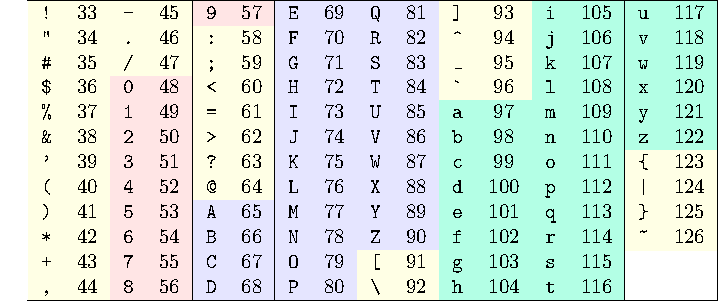
\includegraphics[width=0.9\textwidth]{ascii-table.pdf}
  \caption{All the non-whitespace printable ASCII characters. The four relevant character classes are highlighted in different colours.}
  \label{fig:ascii}
\end{figure}

Of course, the passwords should not be too similar to each other.
Specifically, for every pair of passwords from your list it must be true that they are distinct and that moreover it is not possible to get one from the other by inserting, modifying or deleting a single character.
Formally, the edit distance of any two passwords must be at least $2$.

\begin{Input}
  The input consists of:
  \begin{itemize}
    \item One line with an integer $n$ ($1 \le n \le 1000$), the number of passwords to create.
  \end{itemize}
\end{Input}

\begin{Output}
  Output $n$ lines, each with one password according to the rules above.
  The passwords must have pairwise edit distance at least $2$.
  If there is more than one solution, any one of them will be accepted.
\end{Output}
